\documentclass{article}
\usepackage{tikz}
\usetikzlibrary{patterns}
\usepackage{subcaption}
\usepackage[margin=0.5in]{geometry}

\begin{document}

\begin{figure}[ht]
    \centering
    \begin{subfigure}{0.2375\textwidth}
        \centering
        \resizebox{\textwidth}{!}{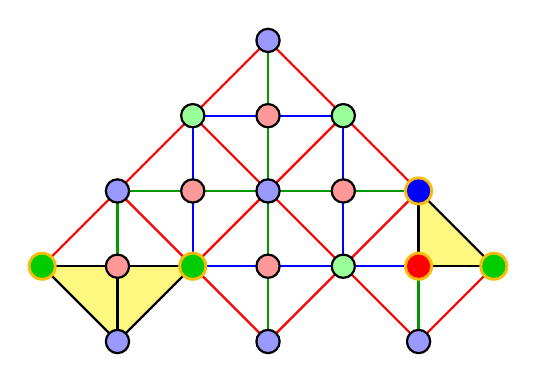
\begin{tikzpicture}[scale=0.7]
    \fill[yellow!50] (-4.0971,1.3657) -- (-2.7314,0.0) -- (-2.7314,1.3657) -- cycle;
    \fill[yellow!50] (-2.7314,0.0) -- (-2.7314,1.3657) -- (-1.3657,1.3657) -- cycle;
    \fill[yellow!50] (2.7314,1.3657) -- (2.7314,2.7314) -- (4.0971,1.3657) -- cycle;
    \draw[black, thick] (2.7314,1.3657) -- (4.0971,1.3657);
    \draw[blue, thick] (1.3657,2.7314) -- (1.3657,1.3657);
    \draw[blue, thick] (-1.3657,2.7314) -- (-1.3657,4.0971);
    \draw[blue, thick] (0.0,1.3657) -- (-1.3657,1.3657);
    \draw[blue, thick] (0.0,4.0971) -- (-1.3657,4.0971);
    \draw[blue, thick] (2.7314,1.3657) -- (1.3657,1.3657);
    \draw[blue, thick] (0.0,1.3657) -- (1.3657,1.3657);
    \draw[blue, thick] (-1.3657,2.7314) -- (-1.3657,1.3657);
    \draw[black, thick] (-2.7314,1.3657) -- (-1.3657,1.3657);
    \draw[blue, thick] (0.0,4.0971) -- (1.3657,4.0971);
    \draw[black, thick] (-2.7314,1.3657) -- (-4.0971,1.3657);
    \draw[blue, thick] (1.3657,2.7314) -- (1.3657,4.0971);
    \draw[red, thick] (-1.3657,4.0971) -- (0.0,5.4628);
    \draw[red, thick] (1.3657,4.0971) -- (0.0,2.7314);
    \draw[black, thick] (4.0971,1.3657) -- (2.7314,2.7314);
    \draw[red, thick] (-1.3657,4.0971) -- (0.0,2.7314);
    \draw[red, thick] (1.3657,1.3657) -- (2.7314,0.0);
    \draw[black, thick] (-1.3657,1.3657) -- (-2.7314,0.0);
    \draw[red, thick] (1.3657,4.0971) -- (2.7314,2.7314);
    \draw[red, thick] (-1.3657,1.3657) -- (0.0,0.0);
    \draw[red, thick] (1.3657,1.3657) -- (0.0,0.0);
    \draw[red, thick] (4.0971,1.3657) -- (2.7314,0.0);
    \draw[red, thick] (1.3657,1.3657) -- (0.0,2.7314);
    \draw[red, thick] (-4.0971,1.3657) -- (-2.7314,2.7314);
    \draw[red, thick] (-1.3657,1.3657) -- (0.0,2.7314);
    \draw[red, thick] (1.3657,4.0971) -- (0.0,5.4628);
    \draw[red, thick] (-1.3657,1.3657) -- (-2.7314,2.7314);
    \draw[red, thick] (1.3657,1.3657) -- (2.7314,2.7314);
    \draw[black, thick] (-4.0971,1.3657) -- (-2.7314,0.0);
    \draw[red, thick] (-1.3657,4.0971) -- (-2.7314,2.7314);
    \draw[green!60!black, thick] (0.0,2.7314) -- (-1.3657,2.7314);
    \draw[green!60!black, thick] (-2.7314,2.7314) -- (-1.3657,2.7314);
    \draw[green!60!black, thick] (0.0,2.7314) -- (0.0,1.3657);
    \draw[green!60!black, thick] (0.0,2.7314) -- (0.0,4.0971);
    \draw[green!60!black, thick] (-2.7314,2.7314) -- (-2.7314,1.3657);
    \draw[green!60!black, thick] (0.0,5.4628) -- (0.0,4.0971);
    \draw[green!60!black, thick] (2.7314,2.7314) -- (1.3657,2.7314);
    \draw[black, thick] (-2.7314,0.0) -- (-2.7314,1.3657);
    \draw[green!60!black, thick] (0.0,2.7314) -- (1.3657,2.7314);
    \draw[green!60!black, thick] (0.0,0.0) -- (0.0,1.3657);
    \draw[black, thick] (2.7314,2.7314) -- (2.7314,1.3657);
    \draw[green!60!black, thick] (2.7314,0.0) -- (2.7314,1.3657);
    \filldraw[fill=blue!40, draw=black, thick] (-2.7314, 0.0) circle (6pt);
    \filldraw[fill=blue!40, draw=black, thick] (0.0, 0.0) circle (6pt);
    \filldraw[fill=blue!40, draw=black, thick] (2.7314, 0.0) circle (6pt);
    \filldraw[fill=blue!40, draw=black, thick] (-2.7314, 2.7314) circle (6pt);
    \filldraw[fill=blue!40, draw=black, thick] (0.0, 2.7314) circle (6pt);
    \filldraw[fill=yellow!50!orange, draw=none] (2.7314, 2.7314) circle (7.5pt);
    \filldraw[fill=blue, draw=none] (2.7314, 2.7314) circle (6pt);
    \filldraw[fill=blue!40, draw=black, thick] (0.0, 5.4628) circle (6pt);
    \filldraw[fill=red!40, draw=black, thick] (-2.7314, 1.3657) circle (6pt);
    \filldraw[fill=red!40, draw=black, thick] (0.0, 1.3657) circle (6pt);
    \filldraw[fill=yellow!50!orange, draw=none] (2.7314, 1.3657) circle (7.5pt);
    \filldraw[fill=red, draw=none] (2.7314, 1.3657) circle (6pt);
    \filldraw[fill=red!40, draw=black, thick] (-1.3657, 2.7314) circle (6pt);
    \filldraw[fill=red!40, draw=black, thick] (1.3657, 2.7314) circle (6pt);
    \filldraw[fill=red!40, draw=black, thick] (0.0, 4.0971) circle (6pt);
    \filldraw[fill=yellow!50!orange, draw=none] (-4.0971, 1.3657) circle (7.5pt);
    \filldraw[fill=green!80!black, draw=none] (-4.0971, 1.3657) circle (6pt);
    \filldraw[fill=yellow!50!orange, draw=none] (-1.3657, 1.3657) circle (7.5pt);
    \filldraw[fill=green!80!black, draw=none] (-1.3657, 1.3657) circle (6pt);
    \filldraw[fill=green!40, draw=black, thick] (1.3657, 1.3657) circle (6pt);
    \filldraw[fill=yellow!50!orange, draw=none] (4.0971, 1.3657) circle (7.5pt);
    \filldraw[fill=green!80!black, draw=none] (4.0971, 1.3657) circle (6pt);
    \filldraw[fill=green!40, draw=black, thick] (-1.3657, 4.0971) circle (6pt);
    \filldraw[fill=green!40, draw=black, thick] (1.3657, 4.0971) circle (6pt);
\end{tikzpicture}
}
        \caption{Full syndrome graph}
    \end{subfigure}
    \hfill
    \begin{subfigure}{0.2375\textwidth}
        \centering
        \resizebox{\textwidth}{!}{\input{restriction_graphs_b.tex}}
        \caption{Red-Green Projection ($\mathcal{L}
    \end{subfigure}
    \hfill
    \begin{subfigure}{0.2375\textwidth}
        \centering
        \resizebox{\textwidth}{!}{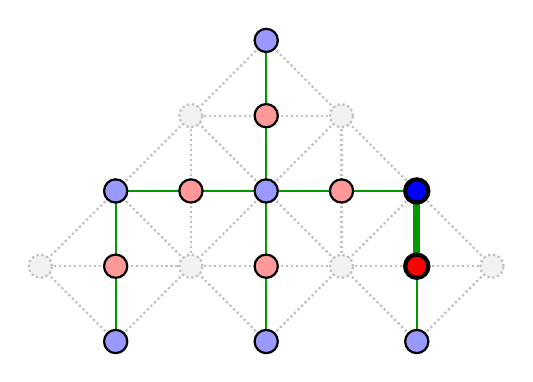
\begin{tikzpicture}[scale=0.7]
    \draw[gray!50, densely dotted, thick] (2.7314,1.3657) -- (4.0971,1.3657);
    \draw[gray!50, densely dotted, thick] (1.3657,2.7314) -- (1.3657,1.3657);
    \draw[gray!50, densely dotted, thick] (-1.3657,2.7314) -- (-1.3657,4.0971);
    \draw[gray!50, densely dotted, thick] (0.0,1.3657) -- (-1.3657,1.3657);
    \draw[gray!50, densely dotted, thick] (0.0,4.0971) -- (-1.3657,4.0971);
    \draw[gray!50, densely dotted, thick] (2.7314,1.3657) -- (1.3657,1.3657);
    \draw[gray!50, densely dotted, thick] (0.0,1.3657) -- (1.3657,1.3657);
    \draw[gray!50, densely dotted, thick] (-1.3657,2.7314) -- (-1.3657,1.3657);
    \draw[gray!50, densely dotted, thick] (-2.7314,1.3657) -- (-1.3657,1.3657);
    \draw[gray!50, densely dotted, thick] (0.0,4.0971) -- (1.3657,4.0971);
    \draw[gray!50, densely dotted, thick] (-2.7314,1.3657) -- (-4.0971,1.3657);
    \draw[gray!50, densely dotted, thick] (1.3657,2.7314) -- (1.3657,4.0971);
    \draw[gray!50, densely dotted, thick] (-1.3657,4.0971) -- (0.0,5.4628);
    \draw[gray!50, densely dotted, thick] (1.3657,4.0971) -- (0.0,2.7314);
    \draw[gray!50, densely dotted, thick] (4.0971,1.3657) -- (2.7314,2.7314);
    \draw[gray!50, densely dotted, thick] (-1.3657,4.0971) -- (0.0,2.7314);
    \draw[gray!50, densely dotted, thick] (1.3657,1.3657) -- (2.7314,0.0);
    \draw[gray!50, densely dotted, thick] (-1.3657,1.3657) -- (-2.7314,0.0);
    \draw[gray!50, densely dotted, thick] (1.3657,4.0971) -- (2.7314,2.7314);
    \draw[gray!50, densely dotted, thick] (-1.3657,1.3657) -- (0.0,0.0);
    \draw[gray!50, densely dotted, thick] (1.3657,1.3657) -- (0.0,0.0);
    \draw[gray!50, densely dotted, thick] (4.0971,1.3657) -- (2.7314,0.0);
    \draw[gray!50, densely dotted, thick] (1.3657,1.3657) -- (0.0,2.7314);
    \draw[gray!50, densely dotted, thick] (-4.0971,1.3657) -- (-2.7314,2.7314);
    \draw[gray!50, densely dotted, thick] (-1.3657,1.3657) -- (0.0,2.7314);
    \draw[gray!50, densely dotted, thick] (1.3657,4.0971) -- (0.0,5.4628);
    \draw[gray!50, densely dotted, thick] (-1.3657,1.3657) -- (-2.7314,2.7314);
    \draw[gray!50, densely dotted, thick] (1.3657,1.3657) -- (2.7314,2.7314);
    \draw[gray!50, densely dotted, thick] (-4.0971,1.3657) -- (-2.7314,0.0);
    \draw[gray!50, densely dotted, thick] (-1.3657,4.0971) -- (-2.7314,2.7314);
    \draw[green!60!black, thick] (0.0,2.7314) -- (-1.3657,2.7314);
    \draw[green!60!black, thick] (-2.7314,2.7314) -- (-1.3657,2.7314);
    \draw[green!60!black, thick] (0.0,2.7314) -- (0.0,1.3657);
    \draw[green!60!black, thick] (0.0,2.7314) -- (0.0,4.0971);
    \draw[green!60!black, thick] (-2.7314,2.7314) -- (-2.7314,1.3657);
    \draw[green!60!black, thick] (0.0,5.4628) -- (0.0,4.0971);
    \draw[green!60!black, thick] (2.7314,2.7314) -- (1.3657,2.7314);
    \draw[green!60!black, thick] (-2.7314,0.0) -- (-2.7314,1.3657);
    \draw[green!60!black, thick] (0.0,2.7314) -- (1.3657,2.7314);
    \draw[green!60!black, thick] (0.0,0.0) -- (0.0,1.3657);
    \draw[green!60!black, line width=2.5pt] (2.7314,2.7314) -- (2.7314,1.3657);
    \draw[green!60!black, thick] (2.7314,0.0) -- (2.7314,1.3657);
    \filldraw[fill=blue!40, draw=black, thick] (-2.7314, 0.0) circle (6pt);
    \filldraw[fill=blue!40, draw=black, thick] (0.0, 0.0) circle (6pt);
    \filldraw[fill=blue!40, draw=black, thick] (2.7314, 0.0) circle (6pt);
    \filldraw[fill=blue!40, draw=black, thick] (-2.7314, 2.7314) circle (6pt);
    \filldraw[fill=blue!40, draw=black, thick] (0.0, 2.7314) circle (6pt);
    \filldraw[fill=blue, draw=black, line width=1.5pt] (2.7314, 2.7314) circle (6pt);
    \filldraw[fill=blue!40, draw=black, thick] (0.0, 5.4628) circle (6pt);
    \filldraw[fill=red!40, draw=black, thick] (-2.7314, 1.3657) circle (6pt);
    \filldraw[fill=red!40, draw=black, thick] (0.0, 1.3657) circle (6pt);
    \filldraw[fill=red, draw=black, line width=1.5pt] (2.7314, 1.3657) circle (6pt);
    \filldraw[fill=red!40, draw=black, thick] (-1.3657, 2.7314) circle (6pt);
    \filldraw[fill=red!40, draw=black, thick] (1.3657, 2.7314) circle (6pt);
    \filldraw[fill=red!40, draw=black, thick] (0.0, 4.0971) circle (6pt);
    \filldraw[fill=gray!10, draw=gray!50, densely dotted, thick] (-4.0971, 1.3657) circle (6pt);
    \filldraw[fill=gray!10, draw=gray!50, densely dotted, thick] (-1.3657, 1.3657) circle (6pt);
    \filldraw[fill=gray!10, draw=gray!50, densely dotted, thick] (1.3657, 1.3657) circle (6pt);
    \filldraw[fill=gray!10, draw=gray!50, densely dotted, thick] (4.0971, 1.3657) circle (6pt);
    \filldraw[fill=gray!10, draw=gray!50, densely dotted, thick] (-1.3657, 4.0971) circle (6pt);
    \filldraw[fill=gray!10, draw=gray!50, densely dotted, thick] (1.3657, 4.0971) circle (6pt);
\end{tikzpicture}
}
        \caption{Red-Blue Projection ($\mathcal{L}
    \end{subfigure}
    \vspace{0.5cm}
    \begin{subfigure}{0.2375\textwidth}
        \centering
        \resizebox{\textwidth}{!}{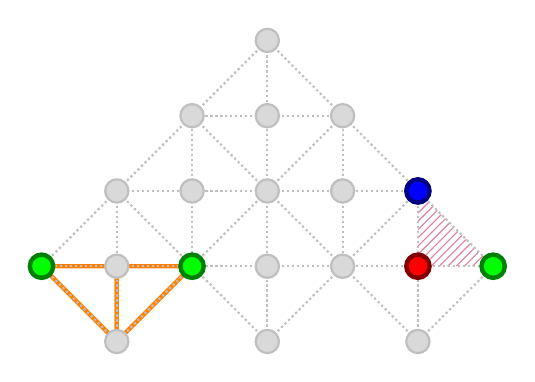
\begin{tikzpicture}[scale=0.7]
    \fill[pattern=north east lines, pattern color=purple!50] (2.7314,1.3657) -- (2.7314,2.7314) -- (4.0971,1.3657) -- cycle;
    \draw[orange, ultra thick] (-4.0971,1.3657) -- (-2.7314,0.0) -- (-2.7314,1.3657) -- cycle;
    \draw[orange, ultra thick] (-2.7314,0.0) -- (-2.7314,1.3657) -- (-1.3657,1.3657) -- cycle;
    \draw[gray!50, densely dotted, thick] (2.7314,1.3657) -- (4.0971,1.3657);
    \draw[gray!50, densely dotted, thick] (1.3657,2.7314) -- (1.3657,1.3657);
    \draw[gray!50, densely dotted, thick] (-1.3657,2.7314) -- (-1.3657,4.0971);
    \draw[gray!50, densely dotted, thick] (0.0,1.3657) -- (-1.3657,1.3657);
    \draw[gray!50, densely dotted, thick] (0.0,4.0971) -- (-1.3657,4.0971);
    \draw[gray!50, densely dotted, thick] (2.7314,1.3657) -- (1.3657,1.3657);
    \draw[gray!50, densely dotted, thick] (0.0,1.3657) -- (1.3657,1.3657);
    \draw[gray!50, densely dotted, thick] (-1.3657,2.7314) -- (-1.3657,1.3657);
    \draw[gray!50, densely dotted, thick] (-2.7314,1.3657) -- (-1.3657,1.3657);
    \draw[gray!50, densely dotted, thick] (0.0,4.0971) -- (1.3657,4.0971);
    \draw[gray!50, densely dotted, thick] (-2.7314,1.3657) -- (-4.0971,1.3657);
    \draw[gray!50, densely dotted, thick] (1.3657,2.7314) -- (1.3657,4.0971);
    \draw[gray!50, densely dotted, thick] (-1.3657,4.0971) -- (0.0,5.4628);
    \draw[gray!50, densely dotted, thick] (1.3657,4.0971) -- (0.0,2.7314);
    \draw[gray!50, densely dotted, thick] (4.0971,1.3657) -- (2.7314,2.7314);
    \draw[gray!50, densely dotted, thick] (-1.3657,4.0971) -- (0.0,2.7314);
    \draw[gray!50, densely dotted, thick] (1.3657,1.3657) -- (2.7314,0.0);
    \draw[gray!50, densely dotted, thick] (-1.3657,1.3657) -- (-2.7314,0.0);
    \draw[gray!50, densely dotted, thick] (1.3657,4.0971) -- (2.7314,2.7314);
    \draw[gray!50, densely dotted, thick] (-1.3657,1.3657) -- (0.0,0.0);
    \draw[gray!50, densely dotted, thick] (1.3657,1.3657) -- (0.0,0.0);
    \draw[gray!50, densely dotted, thick] (4.0971,1.3657) -- (2.7314,0.0);
    \draw[gray!50, densely dotted, thick] (1.3657,1.3657) -- (0.0,2.7314);
    \draw[gray!50, densely dotted, thick] (-4.0971,1.3657) -- (-2.7314,2.7314);
    \draw[gray!50, densely dotted, thick] (-1.3657,1.3657) -- (0.0,2.7314);
    \draw[gray!50, densely dotted, thick] (1.3657,4.0971) -- (0.0,5.4628);
    \draw[gray!50, densely dotted, thick] (-1.3657,1.3657) -- (-2.7314,2.7314);
    \draw[gray!50, densely dotted, thick] (1.3657,1.3657) -- (2.7314,2.7314);
    \draw[gray!50, densely dotted, thick] (-4.0971,1.3657) -- (-2.7314,0.0);
    \draw[gray!50, densely dotted, thick] (-1.3657,4.0971) -- (-2.7314,2.7314);
    \draw[gray!50, densely dotted, thick] (0.0,2.7314) -- (-1.3657,2.7314);
    \draw[gray!50, densely dotted, thick] (-2.7314,2.7314) -- (-1.3657,2.7314);
    \draw[gray!50, densely dotted, thick] (0.0,2.7314) -- (0.0,1.3657);
    \draw[gray!50, densely dotted, thick] (0.0,2.7314) -- (0.0,4.0971);
    \draw[gray!50, densely dotted, thick] (-2.7314,2.7314) -- (-2.7314,1.3657);
    \draw[gray!50, densely dotted, thick] (0.0,5.4628) -- (0.0,4.0971);
    \draw[gray!50, densely dotted, thick] (2.7314,2.7314) -- (1.3657,2.7314);
    \draw[gray!50, densely dotted, thick] (-2.7314,0.0) -- (-2.7314,1.3657);
    \draw[gray!50, densely dotted, thick] (0.0,2.7314) -- (1.3657,2.7314);
    \draw[gray!50, densely dotted, thick] (0.0,0.0) -- (0.0,1.3657);
    \draw[gray!50, densely dotted, thick] (2.7314,2.7314) -- (2.7314,1.3657);
    \draw[gray!50, densely dotted, thick] (2.7314,0.0) -- (2.7314,1.3657);
    \filldraw[fill=gray!30, draw=gray!50, thick] (-2.7314, 0.0) circle (6pt);
    \filldraw[fill=gray!30, draw=gray!50, thick] (0.0, 0.0) circle (6pt);
    \filldraw[fill=gray!30, draw=gray!50, thick] (2.7314, 0.0) circle (6pt);
    \filldraw[fill=gray!30, draw=gray!50, thick] (-2.7314, 2.7314) circle (6pt);
    \filldraw[fill=gray!30, draw=gray!50, thick] (0.0, 2.7314) circle (6pt);
    \filldraw[fill=blue, draw=blue!50!black, ultra thick] (2.7314, 2.7314) circle (6pt);
    \filldraw[fill=gray!30, draw=gray!50, thick] (0.0, 5.4628) circle (6pt);
    \filldraw[fill=gray!30, draw=gray!50, thick] (-2.7314, 1.3657) circle (6pt);
    \filldraw[fill=gray!30, draw=gray!50, thick] (0.0, 1.3657) circle (6pt);
    \filldraw[fill=red, draw=red!50!black, ultra thick] (2.7314, 1.3657) circle (6pt);
    \filldraw[fill=gray!30, draw=gray!50, thick] (-1.3657, 2.7314) circle (6pt);
    \filldraw[fill=gray!30, draw=gray!50, thick] (1.3657, 2.7314) circle (6pt);
    \filldraw[fill=gray!30, draw=gray!50, thick] (0.0, 4.0971) circle (6pt);
    \filldraw[fill=green, draw=green!50!black, ultra thick] (-4.0971, 1.3657) circle (6pt);
    \filldraw[fill=green, draw=green!50!black, ultra thick] (-1.3657, 1.3657) circle (6pt);
    \filldraw[fill=gray!30, draw=gray!50, thick] (1.3657, 1.3657) circle (6pt);
    \filldraw[fill=green, draw=green!50!black, ultra thick] (4.0971, 1.3657) circle (6pt);
    \filldraw[fill=gray!30, draw=gray!50, thick] (-1.3657, 4.0971) circle (6pt);
    \filldraw[fill=gray!30, draw=gray!50, thick] (1.3657, 4.0971) circle (6pt);
\end{tikzpicture}
}
        \caption{Local Lifting}
    \end{subfigure}
    
    \vspace{0.5cm}
    \caption{Full syndrome graph}
\end{figure}

\end{document}